\documentclass[12pt,a4paper,pdflatex]{disser}
\usepackage[russian]{babel}
%\usepackage[utf-8]{inputenc}
%\usepackage{amsmath,amssymb}
%\usepackage{longtable}
\usepackage{parskip}
\usepackage{caption}
\usepackage{textcomp}
\usepackage{gensymb}
\usepackage[dvips]{graphicx}
%\usepackage{wrapfig}
%\usepackage{amssymb}*
%\usepackage{color}
%\usepackage{ulem}
\usepackage{setspace}
\usepackage{hyperref}

\oddsidemargin=-0.5 cm
\evensidemargin=-0.5 cm
\textwidth=170 mm
\textheight=260 mm
\topmargin=0 cm
\voffset= -2cm
\pagenumbering{true}
%\newlength{\varheight}
%\setlength{\varheight}{3.1cm}
\setlength{\parindent}{0cm}
%\newcommand{\taskname}[name]{\begin{center} \bf{\Large{name}} \end{center}}
\spacing{1.1}
\parskip=2mm
\captionsetup[figure]{labelformat=empty}
\clubpenalty=10000
\widowpenalty=10000

\begin{document}

1. Let $\mu$ be the mass of unit length of the rope. Then the net force (in the rotating frame) acting on a small piece $dr$ is
$$
  dF=\left(-\frac{GM}{r^2}+\omega^2 r\right)\mu dr,
$$
where $G=6.67\cdot 10^{-11}$ m^3/(\textrm{kg}\,$\cdot$\,s$^2$) is the gravitational constant, $M=5.97\cdot 10^{24}$ kg is the mass of Earth, $\omega=7.27\cdot 10^{-5}$ rad/s is the frequency of rotation of Earth. Then the net force on the whole rope is
$$
  \frac{F}{\mu}=-GM\left(\frac1R-\frac1{R+L}\right)+\frac{\omega^2}{2}\left((R+L)^2-R^2\right)=\frac{\omega^2 L(L+2R)}{2}-\frac{GML}{R(R+L)},
$$
where $R=6.378\cdot 10^6$ m is the radius of Earth. As the rope hangs free, $F=0$. So,
$$
  \frac{2GM}{\omega^2}=R(R+L)(2R+L),
$$
or, in terms of the geostationary radius $R_0=(GM/\omega^2)^{1/3}$,
$$
  RL^2+3R^2 L+2R^3-2R_0^3=0.
$$
The solution of this equation is
$$
  L=\frac{1}{2R}\left(-3R^2+\sqrt{R_4+8R_0^3 R}\right)=\frac{R}{2}\left(-3+\sqrt{1+\frac{8R_0^3}{R^3}}\right)=1.44\cdot 10^8 \text{ m}.
$$

2. The angular velocity appears to be $\omega=1$, and the radius is $a$. So the linear velocity is $v=\omega a=a$, and the arc length is $l=2\pi a$.

3. Let $x_i$ ($i=1,2,3$) be the displacements of the bodies. Then due to Newton's law
\begin{gather*}
  x_1 ''=\omega_0^2 (x_2-x_1)+ \omega^2 \delta \cos\omega t,\\
  x_2 ''=\omega_0^2 (x_1+x_3-x_2),\\
  x_3 ''=\omega_0^2 (x_2-x_3),
\end{gather*}
where $\omega_0=\sqrt{k/m}$ and $\delta=f/\left(m \omega^2\right)$.
The solution of this system is (obtained by \textit{Mathematica}):
\begin{gather*}
  \xi_1=\frac{x_1}{\delta}=\frac{3\omega^2 \left(\omega^2-3\omega_0^2\right)\cos\omega_0 t -6\left(\omega^4-3\omega_0^2 \omega^2+\omega_0^4\right)\cos\omega t+\left(\omega^2-\omega_0^2\right)\left(2\omega^2-6\omega_0^2+\omega^2 \cos \omega_0 t\sqrt{3}\right)}{6\left(\omega^4-4\omega_0^2 \omega^2+3\omega_0^4\right)},\\
  \xi_2=\frac{x_2}{\delta}=\frac{\omega^2 \left(1-\cos\omega_0 t\sqrt{3}\right)-3\omega_0^2 \left(1-\cos\omega t\right)}{3\left(\omega^2-3\omega_0^2\right)},\\
  \xi_3=\frac{x_3}{\delta}=\frac{6\left(\omega^4-3\omega_0^2 \omega^2+\omega_0^4\right)+\left(\omega^2-\omega_0^2\right)\left(2\omega^2-6\omega_0^2+\omega^2 \cos \omega_0 t\sqrt{3}\right)}{6\left(\omega^4-4\omega_0^2 \omega^2+3\omega_0^4\right)},
\end{gather*}
or, in a dimensionless form with $\varphi=\omega_0 t$ and $\gamma=\omega/\omega_0$,

\begin{gather*}
  \xi_1=\frac{3\gamma^2 \left(\gamma^2-3\right)\cos\varphi -6\left(\gamma^4-3\gamma^2+1\right)\cos\gamma\varphi+\left(\gamma^2-1\right)\left(2\gamma^2-6+\gamma^2 \cos \varphi\sqrt{3}\right)}{6\left(\gamma^4-4\gamma^2+3\right)},\\
  \xi_2=\frac{\gamma^2 \left(1-\cos\varphi\sqrt{3}\right)-3\left(1-\cos\gamma\varphi\right)}{3\left(\gamma^2-3\right)},\\
  \xi_3=\frac{6\left(\gamma^4-3\gamma^2+1\right)+\left(\gamma^2-1\right)\left(2\gamma^2-6+\gamma^2 \cos \varphi\sqrt{3}\right)}{6\left(\gamma^4-4\gamma^2+3\right)}.
\end{gather*}
In case of a resonance $\gamma=1$ this solution is degenerated to
\begin{gather*}
  \xi_1=\frac{1}{12}\left(4-3\cos\varphi-\cos\varphi\sqrt{3}+3\varphi\sin\varphi\right),\\
  \xi_2=\frac{1}{6}\left(2-3\cos\varphi+\cos\varphi\sqrt{3}\right),\\
  \xi_3=\frac{1}{12}\left(4-3\cos\varphi-\cos\varphi\sqrt{3}-3\varphi\sin\varphi\right).
\end{gather*}
There's also a resonance $\gamma=\sqrt3$, in that case
\begin{gather*}
  \xi_1=\frac{1}{12}\left(4+9\cos\varphi-13\cos\varphi\sqrt{3}+\varphi\sqrt3 \sin\varphi\sqrt3\right),\\
  \xi_2=\frac{1}{6}\left(2-2\cos\varphi\sqrt3-\varphi\sqrt{3}\sin\varphi\sqrt3\right),\\
  \xi_3=\frac{1}{12}\left(4-9\cos\varphi+5\cos\varphi\sqrt{3}+\varphi\sqrt3 \sin\varphi\sqrt3\right).
\end{gather*}
The plots of these dependencies are shown below.

\begin{figure}
\begin{center}
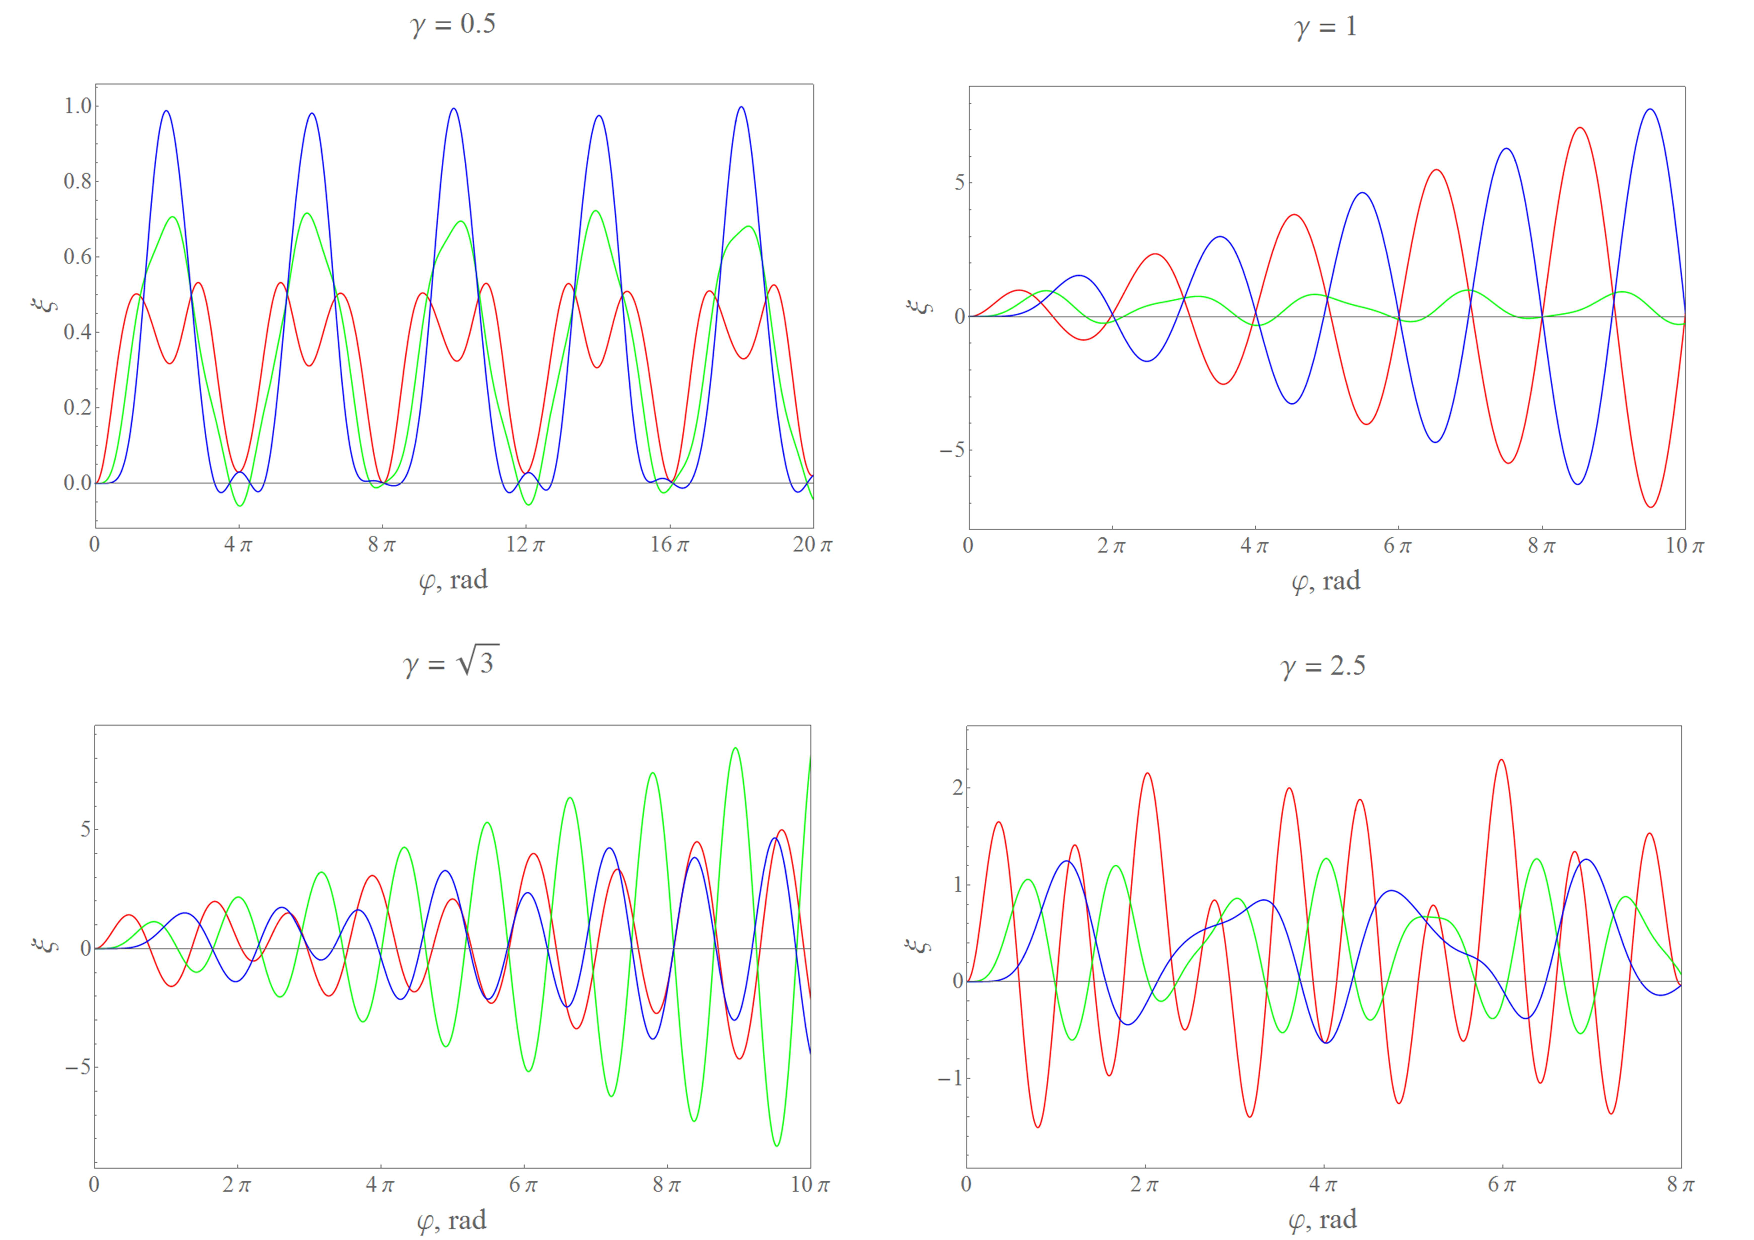
\includegraphics[scale=0.6]{plots.pdf}
\end{center}
\caption{The plots of the $\xi(\varphi)$ dependencies for the bodies, body 1 corresponds to the red curve, body 2 --- to the green, body 3 --- to the blue one.}
\end{figure}

\end{document} 